\section{Aspen Custom Modeler Configuration}
\label{sec.tut.simsinter.acm}
\begin{enumerate}

\item The ``SinterConfigGUI'' can be launched from FOQUS, via the
  \textbf{\underline{Create/Edit}} button found in
  \textbf{\underline{File}}$\rightarrow$ \textbf{\underline{Add/Update Model to
      Turbine}}    or ``SinterConfigGUI'' may be  run on its
  own by selecting \textbf{\underline{SimSinter}} $\rightarrow$ \textbf{\underline{SinterConfigGUI}} from the Start menu.

\item	The splash window displays, as shown in Figure \ref{fig.sinter.acm.splash}. The user may click the splash screen to proceed, or wait ten seconds for it to close automatically.
\begin{figure}[H]
	\begin{center}
		\includegraphics[scale=0.55]{Chapt_sinter/figs/ap/01_Splash_Screen}
		\caption{SinterConfigGUI Splash Screen}
		\label{fig.sinter.acm.splash}
	\end{center}
\end{figure}

\item	The SinterConfigGUI Open Simulation window displays (Figure \ref{fig.sinter.acm.openpage}). If ``SinterConfigGUI'' was
  opened from FOQUS, the filename text box already contains the correct file. To proceed immediately click \textbf{\underline{Open File and Configure Variables}} or click \textbf{\underline{Browse}} to search for the file. For this tutorial, the ACM model for bubbling fluidized bed adsorber installed in the FOQUS examples\textbackslash OUU\textbackslash BFB\_Cap folder is selected (BFB\_OUU\_COE.acmf). Once the file is selected, click \textbf{\underline{Open File and Configure Variables}}. The user can open a fresh ACM simulation (.acmf file) or an existing SimSinter configuration file. For this example, open a fresh simulation.\\
  
  Note: Opening the simulation may take a few minutes depending on how quickly Aspen Custom Modeler can be opened. 
	\begin{figure}[H]
		\begin{center}
			\includegraphics[scale=0.55]{Chapt_sinter/figs/ap/02_FileOpenScreen}
			\caption{SinterConfigGUI Open Simulation Window}
			\label{fig.sinter.acm.openpage}
		\end{center}
	\end{figure}


\item Aspen Custom Modeler starts in the background. This is so the user can observe things about the simulation while working on the configuration file.

\item	The SinterConfigGUI Simulation Meta-Data window displays. (Figure \ref{fig.sinter.acm.savename}). The
  first and most important piece of metadata is \textbf{\underline{SimSinter Save Location}} at
  the top of the window. This is where the sinter configuration file is saved. 
  The system attempts to locate a reasonable file location and file name; however, the user must confirm the correct file location, since it automatically overwrites whatever file name currently exists.
\begin{figure}[H]
	\begin{center}
		\includegraphics[scale=0.55]{Chapt_sinter/figs/acm/03_MetaDataSave}
		\caption{SinterConfigGUI Simulation Meta-Data Page Save Name Text Box}
		\label{fig.sinter.acm.savename}
	\end{center}
\end{figure}

\item Continue to complete the remaining fields and then click
  \textbf{\underline{Next}} (Figure \ref{fig.sinter.acm.metadata}).
\begin{figure}[H]
	\begin{center}
		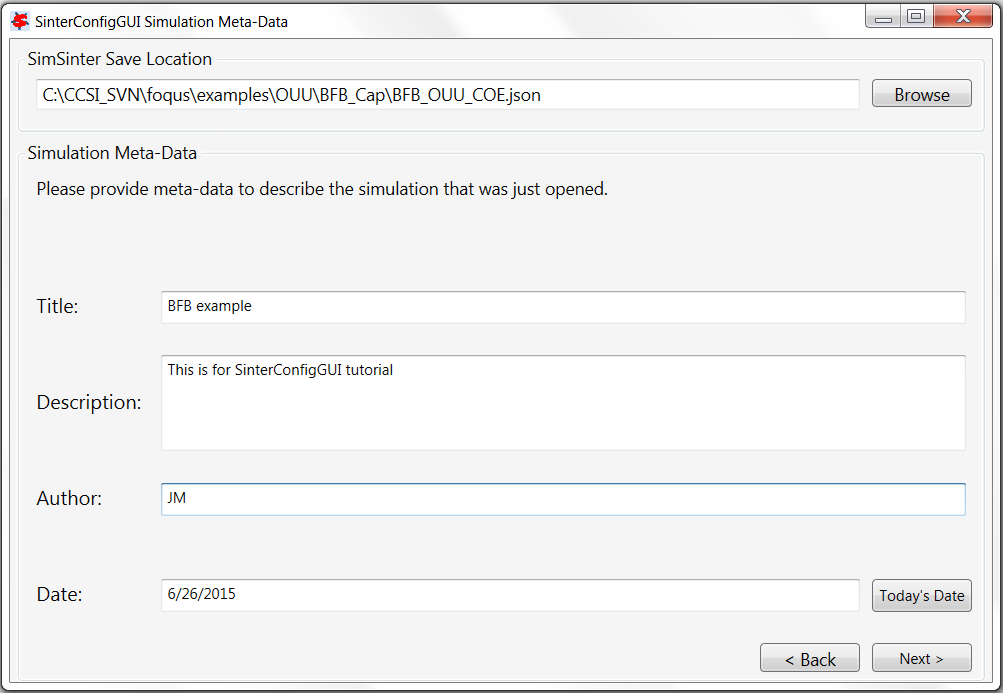
\includegraphics[scale=0.55]{Chapt_sinter/figs/acm/04_MetaDataFilled}
		\caption{SinterConfigGUI Simulation Meta-Data Page with Data Completed}
		\label{fig.sinter.acm.metadata}
	\end{center}
\end{figure}

\item In the \textbf{\underline{SinterConfigGUI Variable Configuration Page}}, (Figure \ref{fig.sinter.acm.variableempty}) notice that the ACM \textbf{\underline{Selected Input Variables}}: \textbf{\underline{TimeSeries}}, \textbf{\underline{Snapshot}}, \textbf{\underline{RunMode}}, \textbf{\underline{printlevel}} and \textbf{\underline{homotopy}} are already included in the input variables.  \textbf{\underline{TimeSeries}} and \textbf{\underline{Snapshot}} are for dynamic simulations. \textbf{\underline{RunMode}} can be either ``Steady State'' or ``Dynamic''. The Dynamic mode requires a dynamic ACM model. For this simulation, the RunMode is Steady State. The \textbf{\underline{homotopy}} variable can be set to ``1'' so that homotopy is on by default.  Notice that the \textbf{\underline{Dynamic}} column (the first column) in each row contains a checkbox, enabling the user to select if the input variable in the row is a dynamic variable.  Also notice that a \textbf{\underline{Variable Type}} search box is on the left. This search is exactly the same as Variable Find on the Tools menu in Aspen Custom Modeler. Please refer to the ACM documentation for details on search patterns.
\begin{figure}[H]
	\begin{center}
		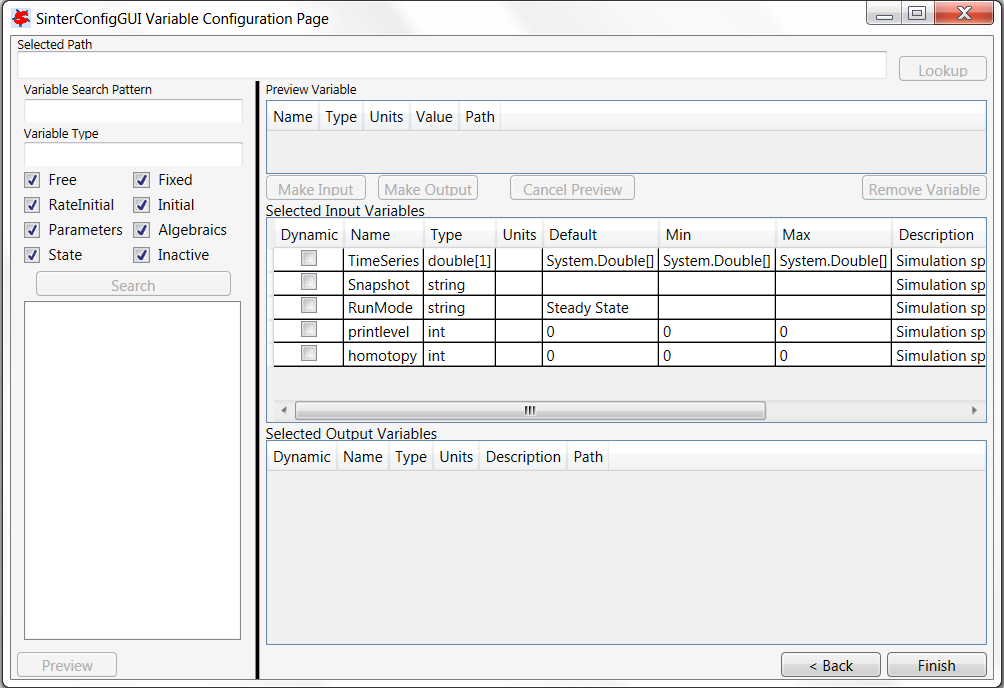
\includegraphics[scale=0.55]{Chapt_sinter/figs/acm/05_VariablesEmpty}
		\caption{SinterConfigGUI Variable Configuration Page before Input}
		\label{fig.sinter.acm.variableempty}
	\end{center}
\end{figure}

\item A search for everything in the ``BFBAdsT'' block has been
  selected. The following \textbf{\underline{Search in Progress}}
  dialog is displayed (Figure \ref{fig.sinter.acm.variableprogress}). Sometimes large searches take a while.
\begin{figure}[H]
	\begin{center}
		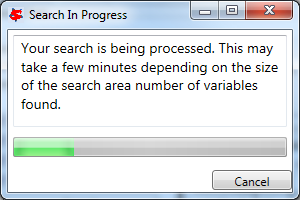
\includegraphics[scale=0.55]{Chapt_sinter/figs/acm/06_Search}
		\caption{Search in Progress Bar Page}
		\label{fig.sinter.acm.variableprogress}
	\end{center}
\end{figure}

\item First, select the ``BFBadsT.A1'' scalar variable in the \textbf{\underline{Selected Path}} field (Figure \ref{fig.sinter.acm.variableselected}).
\begin{figure}[H]
	\begin{center}
		\includegraphics[scale=0.55]{Chapt_sinter/figs/acm/07_VariablesSelected}
		\caption{SinterConfigGUI Variable Configuration Page BFBadsT.A1 Selected}
		\label{fig.sinter.acm.variableselected}
	\end{center}
\end{figure}

\item If the user double-clicks, presses Enter, or clicks \textbf{\underline{Preview}} or \textbf{\underline{Lookup}},
  information displays in the \textbf{\underline{Preview Variable}} section (Figure \ref{fig.sinter.acm.variablepreview}).  Here, the user can verify the variable choices.
\begin{figure}[H]
	\begin{center}
		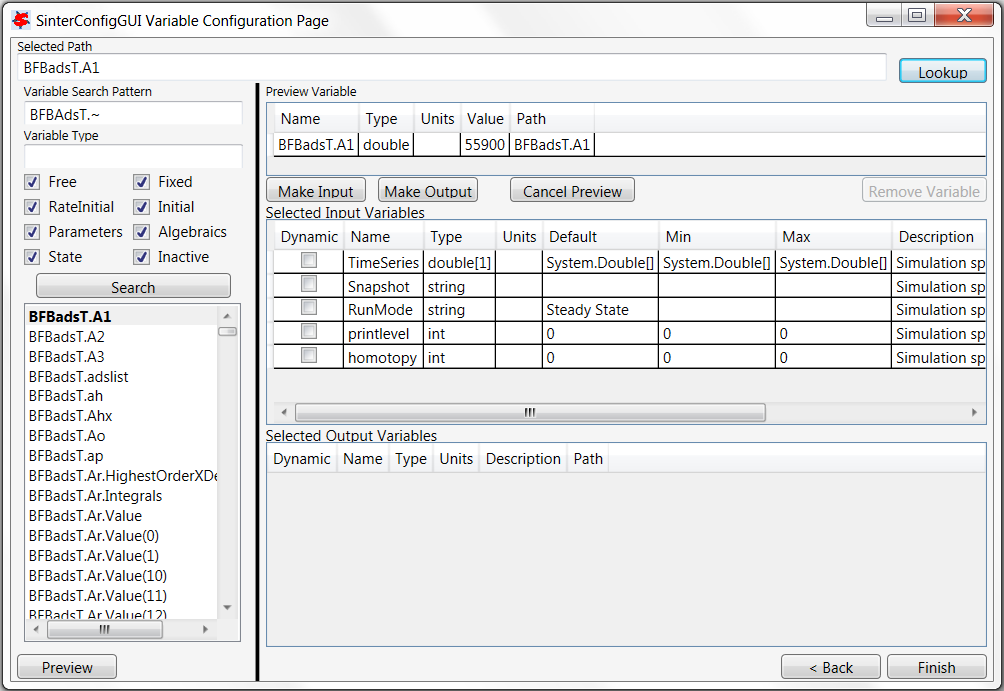
\includegraphics[scale=0.55]{Chapt_sinter/figs/acm/08_VariablePreview}
		\caption{SinterConfigGUI Variable Configuration Page BFBadsT.A1 Preview}
		\label{fig.sinter.acm.variablepreview}
	\end{center}
\end{figure}

\item ``BFBadsT.A1'' is the correct variable; therefore,  click \textbf{\underline{Make Input}}. Information displays in the \textbf{\underline{Selected Input Variables}} section (Figure \ref{fig.sinter.acm.variableinput}).
\begin{figure}[H]
	\begin{center}
		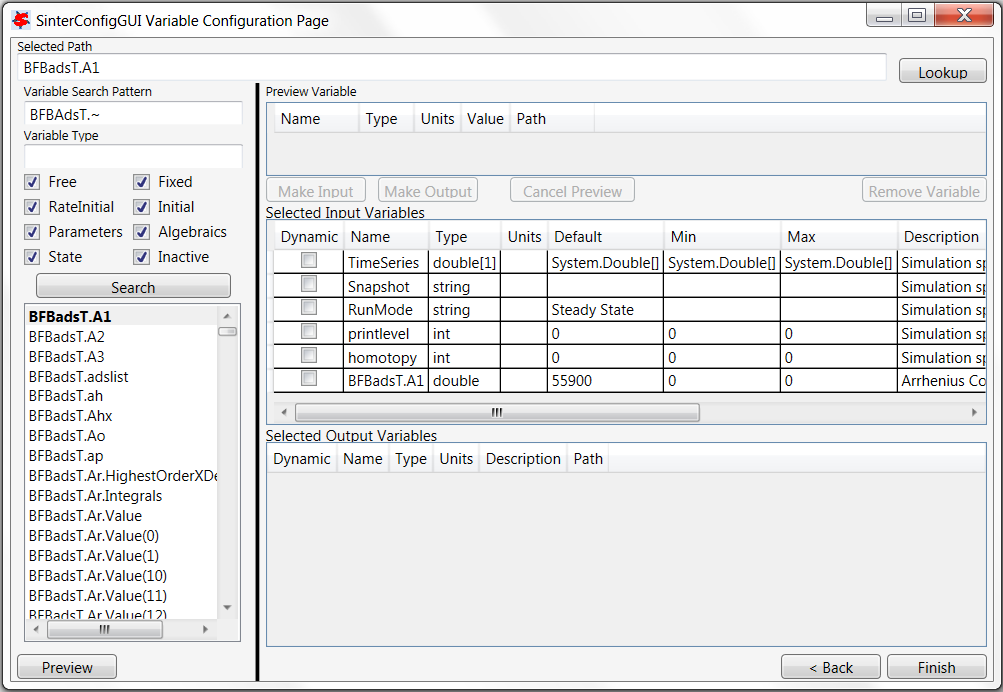
\includegraphics[scale=0.55]{Chapt_sinter/figs/acm/09_VariablesInput}
		\caption{SinterConfigGUI Variable Configuration Page BFBadsT.A1 Made Input}
		\label{fig.sinter.acm.variableinput}
	\end{center}
\end{figure}

\item Change the variable name from ``BFBadsT.A1'' to something more descriptive (e.g., ``WaterA''). Set  \textbf{\underline{Name}}, \textbf{\underline{Description}} and \textbf{\underline{Min/Max}} as shown in Figure \ref{fig.sinter.acm.variablename}.
\begin{figure}[H]
	\begin{center}
		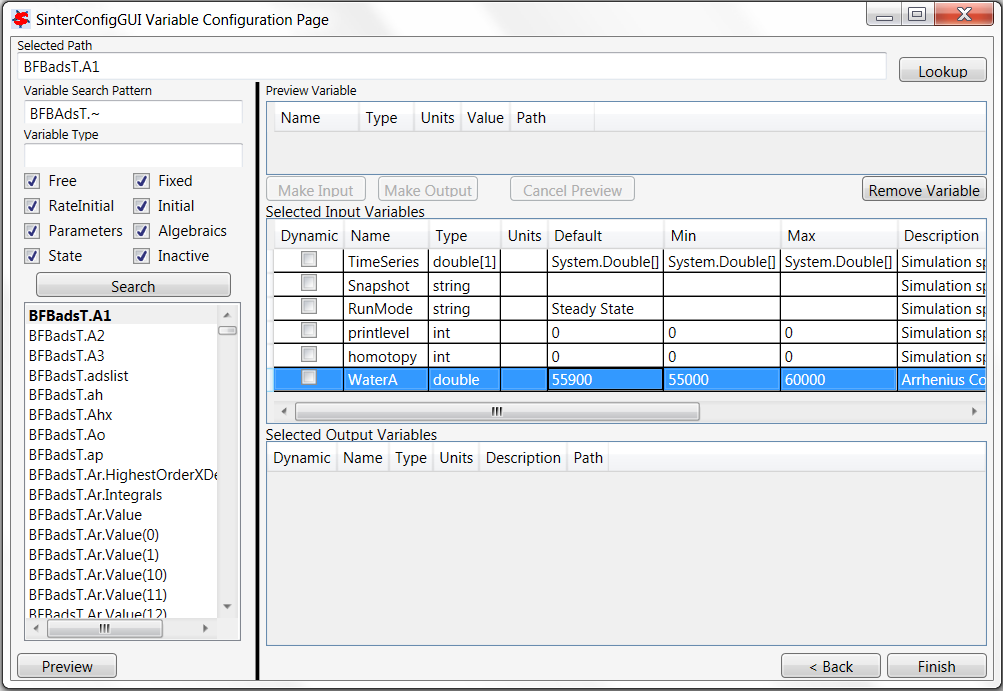
\includegraphics[scale=0.55]{Chapt_sinter/figs/acm/10_VariablesInput2}
		\caption{SinterConfigGUI Variable Configuration Page BFBadsT.A1 Change Name}
		\label{fig.sinter.acm.variablename}
	\end{center}
\end{figure}

\item One input variable is now displayed (Figure \ref{fig.sinter.acm.vectorpreview}). At least one
  output variable is required. In this example, the vector of calculated bubble
  sizes is wanted. Scroll down under \textbf{\underline{Search}} and select ``BFBadsT.db.Value,'' ``BFBadsT.db.Value(0),''
  ``BFBadsT.db.Value(1),'' etc.  If a name with a number in
  parenthesis at the end is selected, it is a specific entry in the vector. If a
  basic name is selected (``BFBadsT.db.Value''), the entire vector is displayed. Select the whole vector and click \textbf{\underline{Preview}}.
\begin{figure}[H]
	\begin{center}
		\includegraphics[scale=0.55]{Chapt_sinter/figs/acm/11_VariablesArray1}
		\caption{SinterConfigGUI Variable Configuration Page Vector Preview}
		\label{fig.sinter.acm.vectorpreview}
	\end{center}
\end{figure}

\item Click \textbf{\underline{Make Output}} if the variable the user wants is selected. Notice that this variable has a unit ``m'' (Figure \ref{fig.sinter.acm.vectoroutput}). 
\begin{figure}[H]
	\begin{center}
		\includegraphics[scale=0.55]{Chapt_sinter/figs/acm/12_VariablesOutput}
		\caption{SinterConfigGUI Variable Configuration Page Vector As Output}
		\label{fig.sinter.acm.vectoroutput}
	\end{center}
\end{figure}

\item Change the \textbf{\underline{Name}} of the variable to ``Diameter.'' Bubble size is measured in meters; however, meters should be converted to millimeters (mm). Now, the output from the simulation should present bubble diameter in mm (Figure \ref{fig.sinter.acm.vectorunits}).  Internal to the simulation, the unit remains ``m.''
\begin{figure}[H]
	\begin{center}
		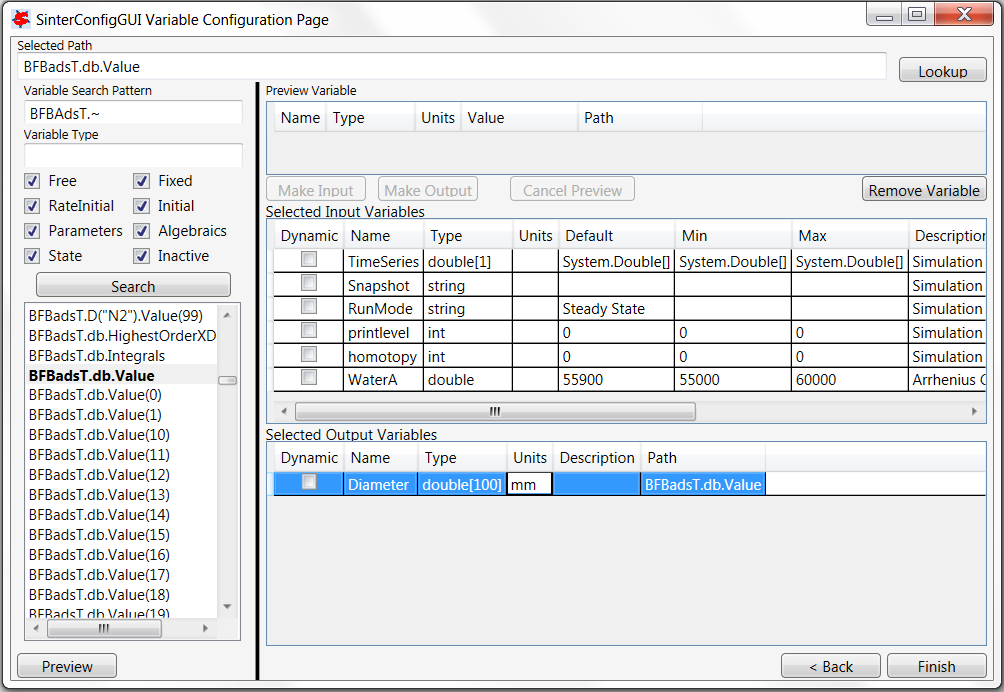
\includegraphics[scale=0.55]{Chapt_sinter/figs/acm/13_VariablesUnits}
		\caption{SinterConfigGUI Variable Configuration Page Output Change Units}
		\label{fig.sinter.acm.vectorunits}
	\end{center}
\end{figure}

\item To add a single item in a vector, select ``BFBadsT.Ar.Value(1)''
  and click \textbf{\underline{Make Input}} (See Figure
  \ref{fig.sinter.acm.vectorremoval}). To remove item that was just added, select it and click \textbf{\underline{Remove Variable}}.
\begin{figure}[H]
	\begin{center}
		\includegraphics[scale=0.55]{Chapt_sinter/figs/acm/14_VariablesInput2}
		\caption{SinterConfigGUI Variable Configuration Page Removal Demo}
		\label{fig.sinter.acm.vectorremoval}
	\end{center}
\end{figure}
%\afterpage\clearpage
\item Select the correct variable vector ``BFBadsT.Ar.Value'' and make it an input (Figure \ref{fig.sinter.acm.vectorreadd}). Notice that a \textbf{\underline{Default}} or \textbf{\underline{Min/Max}} cannot be set in the GUI for a vector. The correct defaults (from the simulation) are set automatically. To change the \textbf{\underline{Min/Max}} values, the user must edit the JSON file in a text editor.
\begin{figure}[H]
	\begin{center}
		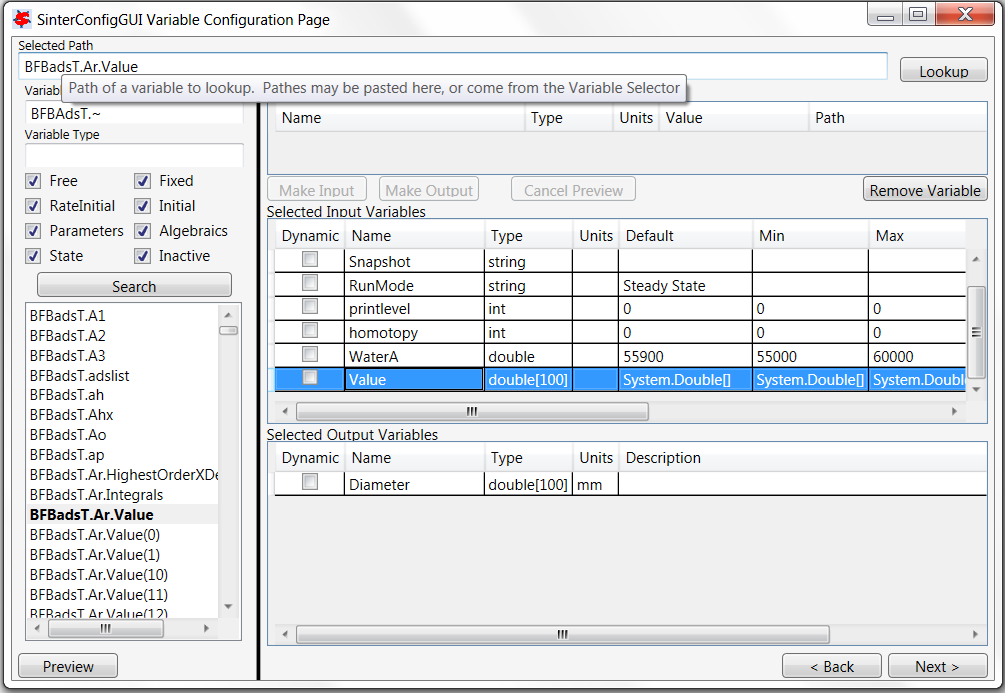
\includegraphics[scale=0.55]{Chapt_sinter/figs/acm/15_VariablesInput4}
		\caption{SinterConfigGUI Variable Configuration Page Read Input}
		\label{fig.sinter.acm.vectorreadd}
	\end{center}
\end{figure}

\item Click \textbf{\underline{Next}} to display the SinterConfigGUI
  Vector Default Initialization window as shown in Figure
  \ref{fig.sinter.acm.vectorinput}. Since the input variable ``Value''
  is a vector, its default values can be modified in the window.  In
  this case there is no need to change the values.
\begin{figure}[H]
	\begin{center}
		\includegraphics[scale=0.55]{Chapt_sinter/figs/acm/16_VectorInput}
		\caption{SinterConfigGUI Vector Default Initialization Input Page}
		\label{fig.sinter.acm.vectorinput}
	\end{center}
\end{figure}
\item The simulation is now setup. Save the configuration file by
  clicking \textbf{\underline{Finish}}. The file is 
  saved to the location specified on the SinterConfigGUI Simulation Meta-Data page. Clicking
  \textbf{\underline{Finish}} will close the SinterConfigGUI, but NOT
  Aspen Custom Modeler.  The user must close ACM manually.

\item If ``SinterConfigGUI'' was launched from FOQUS, the path to the configuration file is
 automatically passed to FOQUS.  The next step in FOQUS is to click
 \textbf{\underline{OK}} in the Add/Update Turbine
     Model window.  FOQUS may then be used to upload it to the Turbine gateway. If ``SinterConfigGUI'' was not launched from FOQUS (e.g., it was
  launched from the Start menu), the configuration file name must be entered in FOQUS manually.
\end{enumerate}
